
\documentclass[tikz,border=10pt]{standalone}

\usepackage{tikz}
\usetikzlibrary{shapes.geometric}

\begin{document}

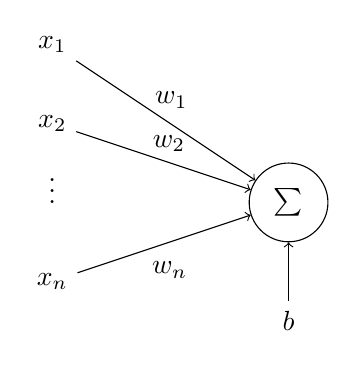
\begin{tikzpicture}[
    neuron/.style={circle, draw, minimum size=1cm}
]

% Input vector (NOT neurons)
\node (X1) at (0,3) {$x_1$};
\node (X2) at (0,2) {$x_2$};
\node at (0,1.25) {\vdots};
\node (Xn) at (0,0) {$x_n$};

\node (B) at (3, -0.5) {$b$};

% Single neuron
\node[neuron] (N) at (3,1) {$\sum$};

% Connection
\draw[->] (X1) -- node[midway, above, yshift=1pt, xshift=2pt] {$w_1$} (N);
\draw[->] (X2) -- node[midway, above, yshift=-0.25pt, xshift=2pt] {$w_2$} (N);
\draw[->] (Xn) -- node[midway, below, yshift=-3pt, xshift=2pt] {$w_n$} (N);

\draw[->] (B) -- (N);

\end{tikzpicture}

\end{document}
